\chapter{Täydellinen haku}

\key{Täydellinen haku}
on yleispätevä tapa ratkaista
lähes mikä tahansa ohjelmointitehtävä.
Ideana on käydä läpi raa'alla voimalla kaikki
mahdolliset tehtävän ratkaisut ja tehtävästä riippuen
valita paras ratkaisu
tai laskea ratkaisuiden yhteismäärä.
          
Täydellinen haku on hyvä menetelmä, jos kaikki
ratkaisut ehtii käydä läpi,
koska haku on yleensä suoraviivainen toteuttaa
ja se antaa varmasti oikean vastauksen.
Jos täydellinen haku on liian hidas,
seuraavien lukujen ahneet algoritmit tai
dynaaminen ohjelmointi voivat soveltua
tehtävään.

\section{Osajoukkojen läpikäynti}

\index{osajoukko@osajoukko}

Aloitamme tapauksesta, jossa tehtävän
mahdollisia ratkaisuja ovat
$n$-alkioisen joukon osajoukot.
Tällöin täydellisen haun tulee
käydä läpi kaikki joukon osa\-joukot,
joita on yhteensä $2^n$ kappaletta.
Käymme seuraavaksi läpi kaksi menetelmää
tällaisen haun toteuttamiseen.

\subsubsection{Menetelmä 1}

Kätevä tapa käydä läpi osajoukot on
käyttää rekursiota.
Seuraava funktio \texttt{haku} muodostaa
joukon $\{1,2,\ldots,n\}$ osajoukot.
Funktio pitää yllä vektoria \texttt{v},
johon se kokoaa osajoukossa olevat luvut.
Osajoukkojen muodostaminen alkaa
tekemällä funktiokutsu \texttt{haku(1)}.

\begin{lstlisting}
void haku(int k) {
    if (k == n+1) {
        // käsittele osajoukko
    } else {
        haku(k+1);
        v.push_back(k);
        haku(k+1);
        v.pop_back();
    }
}
\end{lstlisting}

Funktion parametri $k$ on luku,
joka on ehdolla lisättäväksi osajoukkoon seuraavaksi.
Joka kutsulla funktio haarautuu kahteen tapaukseen:
joko luku $k$ lisätään tai ei lisätä osajoukkoon.
Aina kun $k=n+1$, kaikki luvut on käyty läpi
ja yksi osajoukko on muodostettu.

Esimerkiksi kun $n=3$, funktiokutsut
muodostavat seuraavan kuvan mukaisen puun.
Joka kutsussa 
vasen haara jättää luvun pois osajoukosta
ja oikea haara lisää sen osajoukkoon.
\begin{center}
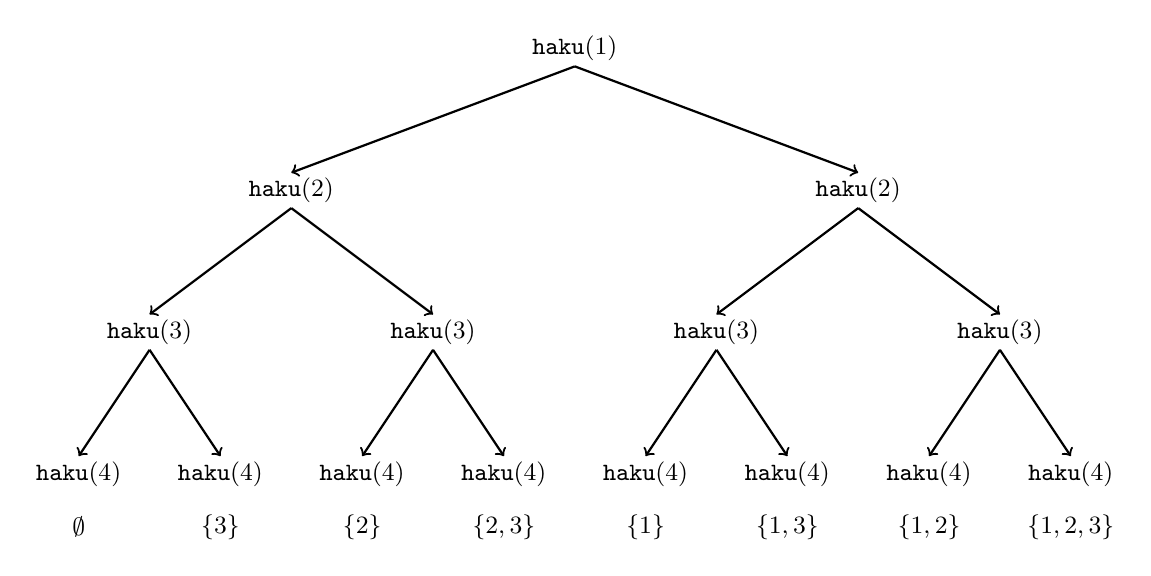
\begin{tikzpicture}[scale=.45]
  \begin{scope}
    \small
    \node at (0,0) {$\texttt{haku}(1)$};

    \node at (-8,-4) {$\texttt{haku}(2)$};
    \node at (8,-4) {$\texttt{haku}(2)$};

    \path[draw,thick,->] (0,0-0.5) -- (-8,-4+0.5);
    \path[draw,thick,->] (0,0-0.5) -- (8,-4+0.5);

    \node at (-12,-8) {$\texttt{haku}(3)$};
    \node at (-4,-8) {$\texttt{haku}(3)$};
    \node at (4,-8) {$\texttt{haku}(3)$};
    \node at (12,-8) {$\texttt{haku}(3)$};

    \path[draw,thick,->] (-8,-4-0.5) -- (-12,-8+0.5);
    \path[draw,thick,->] (-8,-4-0.5) -- (-4,-8+0.5);
    \path[draw,thick,->] (8,-4-0.5) -- (4,-8+0.5);
    \path[draw,thick,->] (8,-4-0.5) -- (12,-8+0.5);

    \node at (-14,-12) {$\texttt{haku}(4)$};
    \node at (-10,-12) {$\texttt{haku}(4)$};
    \node at (-6,-12) {$\texttt{haku}(4)$};
    \node at (-2,-12) {$\texttt{haku}(4)$};
    \node at (2,-12) {$\texttt{haku}(4)$};
    \node at (6,-12) {$\texttt{haku}(4)$};
    \node at (10,-12) {$\texttt{haku}(4)$};
    \node at (14,-12) {$\texttt{haku}(4)$};

    \node at (-14,-13.5) {$\emptyset$};
    \node at (-10,-13.5) {$\{3\}$};
    \node at (-6,-13.5) {$\{2\}$};
    \node at (-2,-13.5) {$\{2,3\}$};
    \node at (2,-13.5) {$\{1\}$};
    \node at (6,-13.5) {$\{1,3\}$};
    \node at (10,-13.5) {$\{1,2\}$};
    \node at (14,-13.5) {$\{1,2,3\}$};


    \path[draw,thick,->] (-12,-8-0.5) -- (-14,-12+0.5);
    \path[draw,thick,->] (-12,-8-0.5) -- (-10,-12+0.5);
    \path[draw,thick,->] (-4,-8-0.5) -- (-6,-12+0.5);
    \path[draw,thick,->] (-4,-8-0.5) -- (-2,-12+0.5);
    \path[draw,thick,->] (4,-8-0.5) -- (2,-12+0.5);
    \path[draw,thick,->] (4,-8-0.5) -- (6,-12+0.5);
    \path[draw,thick,->] (12,-8-0.5) -- (10,-12+0.5);
    \path[draw,thick,->] (12,-8-0.5) -- (14,-12+0.5);
\end{scope}
\end{tikzpicture}
\end{center}

\subsubsection{Menetelmä 2}

Toinen tapa käydä osajoukot läpi on hyödyntää kokonaislukujen
bittiesitystä. Jokainen $n$ alkion osajoukko
voidaan esittää $n$ bitin jonona,
joka taas vastaa lukua väliltä $0 \ldots 2^n-1$.
Bittiesityksen ykkösbitit ilmaisevat,
mitkä joukon alkiot on valittu osajoukkoon.

Tavallinen käytäntö on tulkita kokonaisluvun
bittiesitys osajoukkona niin,
että alkio $k$ kuuluu osajoukkoon,
jos lopusta lukien $k$. bitti on 1.
Esimerkiksi luvun 25 bittiesitys on 11001,
mikä vastaa osajoukkoa $\{1,4,5\}$.

Seuraava koodi käy läpi $n$ alkion joukon
osajoukkojen bittiesitykset:

\begin{lstlisting}
for (int b = 0; b < (1<<n); b++) {
    // käsittele osajoukko b
}
\end{lstlisting}

Seuraava koodi muodostaa jokaisen osajoukon
kohdalla vektorin \texttt{v},
joka sisältää osajoukossa olevat luvut.
Ne saadaan selville tutkimalla, mitkä bitit ovat
ykkösiä osajoukon bittiesityksessä.

\begin{lstlisting}
for (int b = 0; b < (1<<n); b++) {
    vector<int> v;
    for (int i = 0; i < n; i++) {
        if (b&(1<<i)) v.push_back(i+1);
    }
}
\end{lstlisting}

\section{Permutaatioiden läpikäynti}

\index{permutaatio@permutaatio}

Toinen usein esiintyvä tilanne on,
että tehtävän ratkaisut ovat $n$-alkioisen
joukon permutaatioita,
jolloin täydellisen haun tulee
käydä läpi $n!$ mahdollista permutaatiota.
Myös tässä tapauksessa on kaksi luontevaa
menetelmää täydellisen haun toteuttamiseen.

\subsubsection{Menetelmä 1}

Osajoukkojen tavoin permutaatioita voi muodostaa
rekursiivisesti.
Seuraava funktio \texttt{haku} käy läpi
joukon $\{1,2,\ldots,n\}$ permutaatiot.
Funktio muodostaa kunkin permutaation
vuorollaan vektoriin \texttt{v}.
Permutaatioiden muodostus alkaa kutsumalla
funktiota ilman parametreja.

\begin{lstlisting}
void haku() {
    if (v.size() == n) {
        // käsittele permutaatio
    } else {
        for (int i = 1; i <= n; i++) {
            if (p[i]) continue;
            p[i] = 1;
            v.push_back(i);
            haku();
            p[i] = 0;
            v.pop_back();
        }
    }
}
\end{lstlisting}

Funktion jokainen kutsu lisää uuden
luvun permutaatioon vektoriin \texttt{v}.
Taulukko \texttt{p} kertoo, mitkä luvut on jo
valittu permutaatioon.
Jos $\texttt{p}[k]=0$, luku $k$ ei ole mukana,
ja jos $\texttt{p}[k]=1$, luku $k$ on mukana.
Jos vektorin \texttt{v} koko on sama kuin
joukon koko $n$, permutaatio on tullut valmiiksi.

\subsubsection{Menetelmä 2}

\index{next\_permutation@\texttt{next\_permutation}}

Toinen ratkaisu on aloittaa permutaatiosta
$\{1,2,\ldots,n\}$ ja muodostaa joka askeleella
järjestyksessä seuraava permutaatio.
C++:n standardikirjastossa on funktio
\texttt{next\_permutation}, joka tekee tämän muunnoksen.
Seuraava koodi käy läpi joukon $\{1,2,\ldots,n\}$
permutaatiot funktion avulla:

\begin{lstlisting}
vector<int> v;
for (int i = 1; i <= n; i++) {
    v.push_back(i);
}
do {
    // käsittele permutaatio
} while (next_permutation(v.begin(),v.end()));
\end{lstlisting}

\section{Peruuttava haku}

\index{peruuttava haku@peruuttava haku}

\key{Peruuttava haku}
aloittaa ratkaisun etsimisen tyhjästä
ja laajentaa ratkaisua askel kerrallaan.
Joka askeleella haku haarautuu kaikkiin
mahdollisiin suuntiin, joihin ratkaisua voi laajentaa.
Haaran tutkimisen jälkeen haku peruuttaa takaisin
ja jatkaa muihin mahdollisiin suuntiin.

\index{kuningatarongelma}

Tarkastellaan esimerkkinä \key{kuningatarongelmaa},
jossa laskettavana on,
monellako tavalla $n \times n$ -shakkilaudalle
voidaan asettaa $n$ kuningatarta niin,
että mitkään kaksi kuningatarta eivät uhkaa toisiaan.
Esimerkiksi kun $n=4$, mahdolliset ratkaisut ovat seuraavat:

\begin{center}
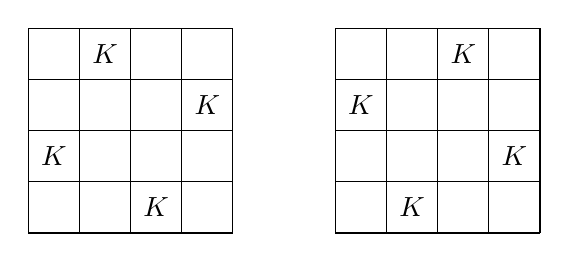
\begin{tikzpicture}[scale=.65]
  \begin{scope}
    \draw (0, 0) grid (4, 4);
    \node at (1.5,3.5) {$K$};
    \node at (3.5,2.5) {$K$};
    \node at (0.5,1.5) {$K$};
    \node at (2.5,0.5) {$K$};

    \draw (6, 0) grid (10, 4);
    \node at (6+2.5,3.5) {$K$};
    \node at (6+0.5,2.5) {$K$};
    \node at (6+3.5,1.5) {$K$};
    \node at (6+1.5,0.5) {$K$};

  \end{scope}
\end{tikzpicture}
\end{center}

Tehtävän voi ratkaista peruuttavalla haulla
muodostamalla ratkaisua rivi kerrallaan.
Jokaisella rivillä täytyy valita yksi ruuduista,
johon sijoitetaan kuningatar niin,
ettei se uhkaa mitään aiemmin lisättyä kuningatarta.
Ratkaisu on valmis, kun viimeisellekin
riville on lisätty kuningatar.

Esimerkiksi kun $n=4$, osa peruuttavan haun muodostamasta
puusta näyttää seuraavalta:

\begin{center}
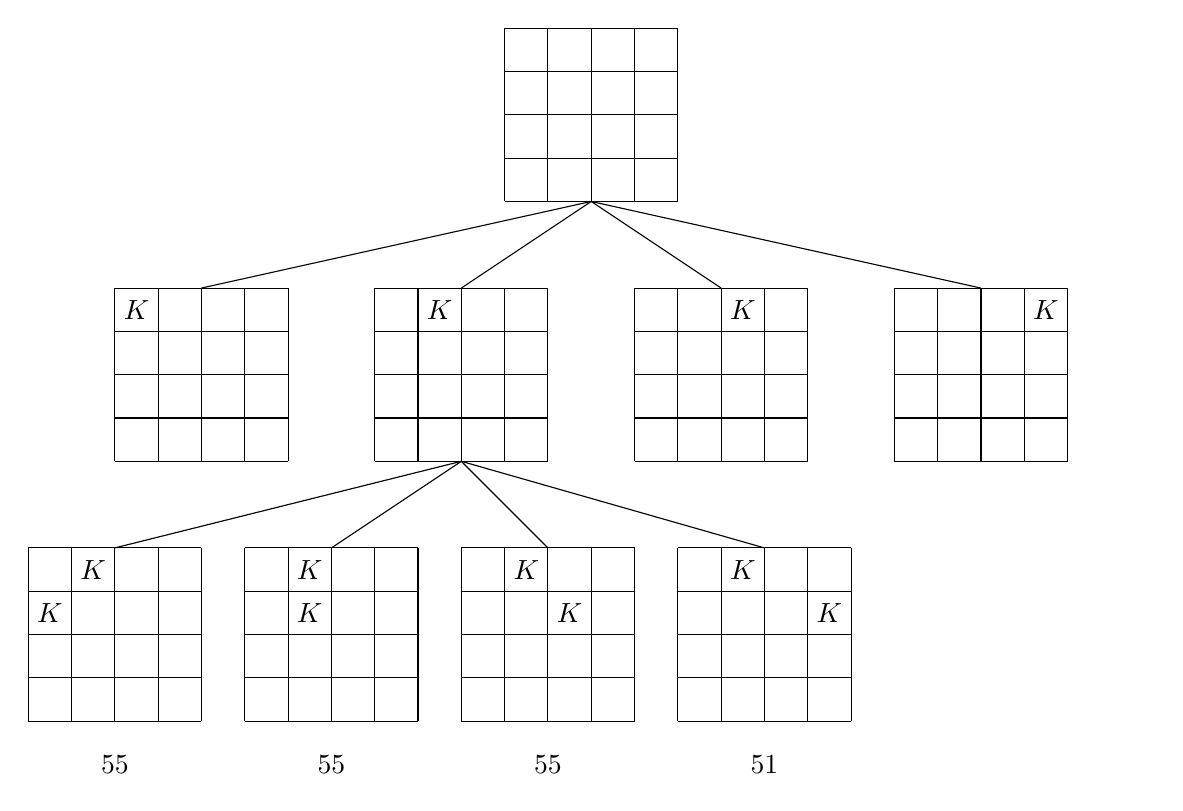
\begin{tikzpicture}[scale=.55]
  \begin{scope}
    \draw (0, 0) grid (4, 4);

    \draw (-9, -6) grid (-5, -2);
    \draw (-3, -6) grid (1, -2);
    \draw (3, -6) grid (7, -2);
    \draw (9, -6) grid (13, -2);

    \node at (-9+0.5,-3+0.5) {$K$};
    \node at (-3+1+0.5,-3+0.5) {$K$};
    \node at (3+2+0.5,-3+0.5) {$K$};
    \node at (9+3+0.5,-3+0.5) {$K$};

    \draw (2,0) -- (-7,-2);
    \draw (2,0) -- (-1,-2);
    \draw (2,0) -- (5,-2);
    \draw (2,0) -- (11,-2);

    \draw (-11, -12) grid (-7, -8);
    \draw (-6, -12) grid (-2, -8);
    \draw (-1, -12) grid (3, -8);
    \draw (4, -12) grid (8, -8);
    \draw[white] (11, -12) grid (15, -8);
    \node at (-11+1+0.5,-9+0.5) {$K$};
    \node at (-6+1+0.5,-9+0.5) {$K$};
    \node at (-1+1+0.5,-9+0.5) {$K$};
    \node at (4+1+0.5,-9+0.5) {$K$};
    \node at (-11+0+0.5,-10+0.5) {$K$};
    \node at (-6+1+0.5,-10+0.5) {$K$};
    \node at (-1+2+0.5,-10+0.5) {$K$};
    \node at (4+3+0.5,-10+0.5) {$K$};

    \draw (-1,-6) -- (-9,-8);
    \draw (-1,-6) -- (-4,-8);
    \draw (-1,-6) -- (1,-8);
    \draw (-1,-6) -- (6,-8);

    \node at (-9,-13) {\ding{55}};
    \node at (-4,-13) {\ding{55}};
    \node at (1,-13) {\ding{55}};
    \node at (6,-13) {\ding{51}};

  \end{scope}
\end{tikzpicture}
\end{center}

Kuvan alimmalla tasolla kolme ensimmäistä osaratkaisua
eivät kelpaa, koska niissä kuningattaret uhkaavat
toisiaan.
Sen sijaan neljäs osaratkaisu kelpaa,
ja sitä on mahdollista laajentaa loppuun asti
kokonaiseksi ratkaisuksi
asettamalla kaksi kuningatarta lisää laudalle.

\begin{samepage}
Seuraava koodi toteuttaa peruuttavan haun:

\begin{lstlisting}
void haku(int y) {
    if (y == n) {
        c++;
        return;
    }
    for (int x = 0; x < n; x++) {
        if (r1[x] || r2[x+y] || r3[x-y+n-1]) continue;
        r1[x] = r2[x+y] = r3[x-y+n-1] = 1;
        haku(y+1);
        r1[x] = r2[x+y] = r3[x-y+n-1] = 0;
    }
}
\end{lstlisting}
\end{samepage}
Haku alkaa kutsumalla funktiota \texttt{haku(0)}.
Laudan koko on muuttujassa $n$,
ja koodi laskee ratkaisuiden määrän
muuttujaan $c$.

Koodi olettaa, että laudan vaaka- ja pystyrivit
on numeroitu 0:sta alkaen.
Funktio asettaa kuningattaren vaakariville $y$,
kun $0 \le y < n$.
Jos taas $y=n$, yksi ratkaisu on valmis
ja funktio kasvattaa muuttujaa $c$.

Taulukko \texttt{r1} pitää kirjaa,
millä laudan pystyriveillä on jo kuningatar.
Vastaavasti taulukot \texttt{r2} ja \texttt{r3}
pitävät kirjaa vinoriveistä.
Tällaisille riveille ei voi laittaa enää toista
kuningatarta.
Esimerkiksi $4 \times 4$ -laudan tapauksessa
rivit on numeroitu seuraavasti:

\begin{center}
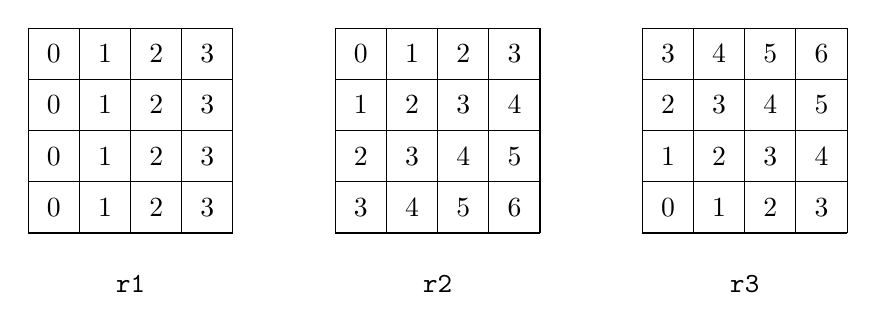
\begin{tikzpicture}[scale=.65]
  \begin{scope}
    \draw (0-6, 0) grid (4-6, 4);
    \node at (-6+0.5,3.5) {$0$};
    \node at (-6+1.5,3.5) {$1$};
    \node at (-6+2.5,3.5) {$2$};
    \node at (-6+3.5,3.5) {$3$};
    \node at (-6+0.5,2.5) {$0$};
    \node at (-6+1.5,2.5) {$1$};
    \node at (-6+2.5,2.5) {$2$};
    \node at (-6+3.5,2.5) {$3$};
    \node at (-6+0.5,1.5) {$0$};
    \node at (-6+1.5,1.5) {$1$};
    \node at (-6+2.5,1.5) {$2$};
    \node at (-6+3.5,1.5) {$3$};
    \node at (-6+0.5,0.5) {$0$};
    \node at (-6+1.5,0.5) {$1$};
    \node at (-6+2.5,0.5) {$2$};
    \node at (-6+3.5,0.5) {$3$};

    \draw (0, 0) grid (4, 4);
    \node at (0.5,3.5) {$0$};
    \node at (1.5,3.5) {$1$};
    \node at (2.5,3.5) {$2$};
    \node at (3.5,3.5) {$3$};
    \node at (0.5,2.5) {$1$};
    \node at (1.5,2.5) {$2$};
    \node at (2.5,2.5) {$3$};
    \node at (3.5,2.5) {$4$};
    \node at (0.5,1.5) {$2$};
    \node at (1.5,1.5) {$3$};
    \node at (2.5,1.5) {$4$};
    \node at (3.5,1.5) {$5$};
    \node at (0.5,0.5) {$3$};
    \node at (1.5,0.5) {$4$};
    \node at (2.5,0.5) {$5$};
    \node at (3.5,0.5) {$6$};

    \draw (6, 0) grid (10, 4);
    \node at (6.5,3.5) {$3$};
    \node at (7.5,3.5) {$4$};
    \node at (8.5,3.5) {$5$};
    \node at (9.5,3.5) {$6$};
    \node at (6.5,2.5) {$2$};
    \node at (7.5,2.5) {$3$};
    \node at (8.5,2.5) {$4$};
    \node at (9.5,2.5) {$5$};
    \node at (6.5,1.5) {$1$};
    \node at (7.5,1.5) {$2$};
    \node at (8.5,1.5) {$3$};
    \node at (9.5,1.5) {$4$};
    \node at (6.5,0.5) {$0$};
    \node at (7.5,0.5) {$1$};
    \node at (8.5,0.5) {$2$};
    \node at (9.5,0.5) {$3$};

    \node at (-4,-1) {\texttt{r1}};
    \node at (2,-1) {\texttt{r2}};
    \node at (8,-1) {\texttt{r3}};

  \end{scope}
\end{tikzpicture}
\end{center}

Koodin avulla selviää esimerkiksi,
että tapauksessa $n=8$ on 92 tapaa sijoittaa 8
kuningatarta $8 \times 8$ -laudalle.
Kun $n$ kasvaa, koodi hidastuu nopeasti,
koska ratkaisujen määrä kasvaa räjähdysmäisesti.
Tapauksen $n=16$ laskeminen vie jo noin minuutin
nykyaikaisella tietokoneella (14772512 ratkaisua).

\section{Haun optimointi}

Peruuttavaa hakua on usein mahdollista tehostaa
erilaisten optimointien avulla.
Ideana on lisätä hakuun ''älykkyyttä''
niin, että haku pystyy havaitsemaan
mahdollisimman aikaisin,
jos muodosteilla oleva ratkaisu ei voi
johtaa kokonaiseen ratkaisuun.
Tällaiset optimoinnit karsivat haaroja
hakupuusta, millä voi olla suuri vaikutus
peruuttavan haun tehokkuuteen.

Tarkastellaan esimerkkinä tehtävää,
jossa laskettavana on reittien määrä
$n \times n$ -ruudukon
vasemmasta yläkulmasta oikeaan alakulmaan,
kun reitin aikana tulee käydä tarkalleen kerran 
jokaisessa ruudussa.
Esimerkiksi $7 \times 7$ -ruudukossa on
111712 mahdollista reittiä vasemmasta yläkulmasta
oikeaan alakulmaan, joista yksi on seuraava:

\begin{center}
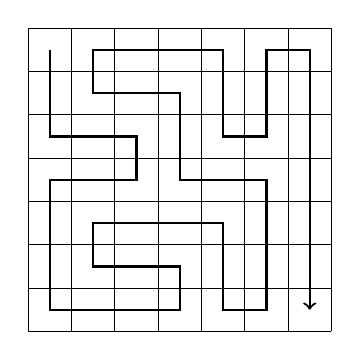
\begin{tikzpicture}[scale=.55]
  \begin{scope}
    \draw (0, 0) grid (7, 7);
    \draw[thick,->] (0.5,6.5) -- (0.5,4.5) -- (2.5,4.5) --
          (2.5,3.5) -- (0.5,3.5) -- (0.5,0.5) --
          (3.5,0.5) -- (3.5,1.5) -- (1.5,1.5) --
          (1.5,2.5) -- (4.5,2.5) -- (4.5,0.5) --
          (5.5,0.5) -- (5.5,3.5) -- (3.5,3.5) --
          (3.5,5.5) -- (1.5,5.5) -- (1.5,6.5) --
          (4.5,6.5) -- (4.5,4.5) -- (5.5,4.5) --
          (5.5,6.5) -- (6.5,6.5) -- (6.5,0.5);
  \end{scope}
\end{tikzpicture}
\end{center}

Keskitymme seuraavaksi nimenomaan tapaukseen $7 \times 7$,
koska se on laskennallisesti sopivan haastava.
Lähdemme liikkeelle suoraviivaisesta peruuttavaa hakua
käyttävästä algoritmista
ja teemme siihen pikkuhiljaa optimointeja,
jotka nopeuttavat hakua eri tavoin.
Mittaamme jokaisen optimoinnin jälkeen
algoritmin suoritusajan sekä rekursiokutsujen yhteismäärän,
jotta näemme selvästi, mikä vaikutus kullakin
optimoinnilla on haun tehokkuuteen.

\subsubsection{Perusalgoritmi}

Algoritmin ensimmäisessä versiossa ei ole mitään optimointeja,
vaan peruuttava haku käy läpi kaikki mahdolliset tavat
muodostaa reitti ruudukon vasemmasta yläkulmasta
oikeaan alakulmaan.

\begin{itemize}
\item
suoritusaika: 483 sekuntia
\item
rekursiokutsuja: 76 miljardia
\end{itemize}

\subsubsection{Optimointi 1}

Reitin ensimmäinen askel on joko alaspäin
tai oikealle. Tästä valinnasta seuraavat tilanteet
ovat symmetrisiä ruudukon lävistäjän suhteen.
Esimerkiksi seuraavat ratkaisut ovat
symmetrisiä keskenään:

\begin{center}
\begin{tabular}{ccc}
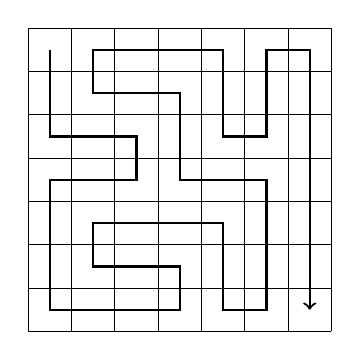
\begin{tikzpicture}[scale=.55]
  \begin{scope}
    \draw (0, 0) grid (7, 7);
    \draw[thick,->] (0.5,6.5) -- (0.5,4.5) -- (2.5,4.5) --
          (2.5,3.5) -- (0.5,3.5) -- (0.5,0.5) --
          (3.5,0.5) -- (3.5,1.5) -- (1.5,1.5) --
          (1.5,2.5) -- (4.5,2.5) -- (4.5,0.5) --
          (5.5,0.5) -- (5.5,3.5) -- (3.5,3.5) --
          (3.5,5.5) -- (1.5,5.5) -- (1.5,6.5) --
          (4.5,6.5) -- (4.5,4.5) -- (5.5,4.5) --
          (5.5,6.5) -- (6.5,6.5) -- (6.5,0.5);
  \end{scope}
\end{tikzpicture}
& \hspace{20px}
& 
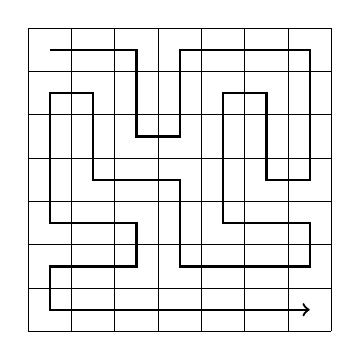
\begin{tikzpicture}[scale=.55]
  \begin{scope}[yscale=1,xscale=-1,rotate=-90]
    \draw (0, 0) grid (7, 7);
    \draw[thick,->] (0.5,6.5) -- (0.5,4.5) -- (2.5,4.5) --
          (2.5,3.5) -- (0.5,3.5) -- (0.5,0.5) --
          (3.5,0.5) -- (3.5,1.5) -- (1.5,1.5) --
          (1.5,2.5) -- (4.5,2.5) -- (4.5,0.5) --
          (5.5,0.5) -- (5.5,3.5) -- (3.5,3.5) --
          (3.5,5.5) -- (1.5,5.5) -- (1.5,6.5) --
          (4.5,6.5) -- (4.5,4.5) -- (5.5,4.5) --
          (5.5,6.5) -- (6.5,6.5) -- (6.5,0.5);
  \end{scope}
\end{tikzpicture}
\end{tabular}
\end{center}

Tämän ansiosta voimme tehdä päätöksen,
että reitin ensimmäinen askel on alaspäin,
ja kertoa lopuksi reittien määrän 2:lla.

\begin{itemize}
\item
suoritusaika: 244 sekuntia
\item
rekursiokutsuja: 38 miljardia
\end{itemize}

\subsubsection{Optimointi 2}

Jos reitti menee oikean alakulman ruutuun ennen kuin
se on käynyt kaikissa muissa ruuduissa,
siitä ei voi mitenkään enää saada kelvollista ratkaisua.
Näin on esimerkiksi seuraavassa tilanteessa:

\begin{center}
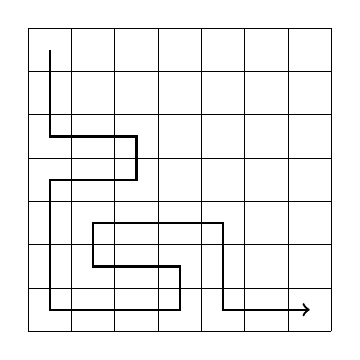
\begin{tikzpicture}[scale=.55]
  \begin{scope}
    \draw (0, 0) grid (7, 7);
    \draw[thick,->] (0.5,6.5) -- (0.5,4.5) -- (2.5,4.5) --
          (2.5,3.5) -- (0.5,3.5) -- (0.5,0.5) --
          (3.5,0.5) -- (3.5,1.5) -- (1.5,1.5) --
          (1.5,2.5) -- (4.5,2.5) -- (4.5,0.5) --
          (6.5,0.5);
  \end{scope}
\end{tikzpicture}
\end{center}
Niinpä voimme keskeyttää hakuhaaran heti,
jos tulemme oikean alakulman ruutuun liian aikaisin.
\begin{itemize}
\item
suoritusaika: 119 sekuntia
\item
rekursiokutsuja: 20 miljardia
\end{itemize}

\subsubsection{Optimointi 3}

Jos reitti osuu seinään niin, että kummallakin puolella
on ruutu, jossa reitti ei ole vielä käynyt,
ruudukko jakautuu kahteen osaan.
Esimerkiksi seuraavassa tilanteessa
sekä vasemmalla että
oikealla puolella on tyhjä ruutu:

\begin{center}
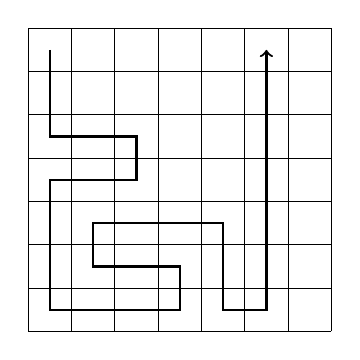
\begin{tikzpicture}[scale=.55]
  \begin{scope}
    \draw (0, 0) grid (7, 7);
    \draw[thick,->] (0.5,6.5) -- (0.5,4.5) -- (2.5,4.5) --
          (2.5,3.5) -- (0.5,3.5) -- (0.5,0.5) --
          (3.5,0.5) -- (3.5,1.5) -- (1.5,1.5) --
          (1.5,2.5) -- (4.5,2.5) -- (4.5,0.5) --
          (5.5,0.5) -- (5.5,6.5);
  \end{scope}
\end{tikzpicture}
\end{center}
Nyt ei ole enää mahdollista käydä kaikissa ruuduissa,
joten voimme keskeyttää hakuhaaran.
Tämä optimointi on hyvin hyödyllinen:

\begin{itemize}
\item
suoritusaika: 1{,}8 sekuntia
\item
rekursiokutsuja: 221 miljoonaa
\end{itemize}

\subsubsection{Optimointi 4}

Äskeisen optimoinnin ideaa voi yleistää:
ruudukko jakaantuu kahteen osaan,
jos nykyisen ruudun ylä- ja alapuolella on
tyhjä ruutu sekä vasemmalla ja oikealla
puolella on seinä tai aiemmin käyty ruutu
(tai päinvastoin).

Esimerkiksi seuraavassa tilanteessa
nykyisen ruudun ylä- ja alapuolella on
tyhjä ruutu eikä reitti voi enää edetä
molempiin ruutuihin:
\begin{center}
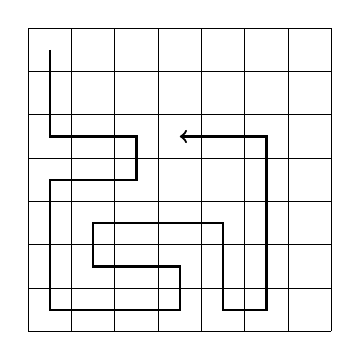
\begin{tikzpicture}[scale=.55]
  \begin{scope}
    \draw (0, 0) grid (7, 7);
    \draw[thick,->] (0.5,6.5) -- (0.5,4.5) -- (2.5,4.5) --
          (2.5,3.5) -- (0.5,3.5) -- (0.5,0.5) --
          (3.5,0.5) -- (3.5,1.5) -- (1.5,1.5) --
          (1.5,2.5) -- (4.5,2.5) -- (4.5,0.5) --
          (5.5,0.5) -- (5.5,4.5) -- (3.5,4.5);
  \end{scope}
\end{tikzpicture}
\end{center}
Haku tehostuu entisestään, kun keskeytämme
hakuhaaran kaikissa tällaisissa tapauksissa:

\begin{itemize}
\item
suoritusaika: 0{,}6 sekuntia
\item
rekursiokutsuja: 69 miljoonaa
\end{itemize}

~\\
Nyt on hyvä hetki lopettaa optimointi ja muistella,
mistä lähdimme liikkeelle.
Alkuperäinen algoritmi vei aikaa 483 sekuntia,
ja nyt optimointien jälkeen algoritmi vie aikaa
vain 0{,}6 sekuntia.
Optimointien ansiosta algoritmi nopeutui
siis lähes 1000-kertaisesti.

Tämä on yleinen ilmiö peruuttavassa haussa,
koska hakupuu on yleensä valtava ja
yksinkertainenkin optimointi voi karsia suuren
määrän haaroja hakupuusta.
Erityisen hyödyllisiä ovat optimoinnit,
jotka kohdistuvat hakupuun yläosaan,
koska ne karsivat eniten haaroja.

\section{Puolivälihaku}

\index{puolivxlihaku@puolivälihaku}

\key{Puolivälihaku} (''meet in the middle'') on tekniikka,
jossa hakutehtävä jaetaan kahteen yhtä suureen osaan.
Kumpaankin osaan tehdään erillinen haku,
ja lopuksi hakujen tulokset yhdistetään.

Puolivälihaun käyttäminen edellyttää,
että erillisten hakujen tulokset pystyy
yhdistämään tehokkaasti.
Tällöin puolivälihaku on tehokkaampi
kuin yksi haku, joka käy läpi koko hakualueen.
Tyypillisesti puolivälihaku tehostaa algoritmia
niin, että aikavaativuuden kertoimesta $2^n$
tulee kerroin $2^{n/2}$.

Tarkastellaan ongelmaa, jossa annettuna
on $n$ lukua sisältävä lista sekä kokonaisluku $x$.
Tehtävänä on selvittää, voiko listalta valita
joukon lukuja niin, että niiden summa on $x$.
Esimerkiksi jos lista on $[2,4,5,9]$ ja $x=15$,
voimme valita listalta luvut $[2,4,9]$,
jolloin $2+4+9=15$.
Jos taas lista säilyy ennallaan ja $x=14$,
mikään valinta ei täytä vaatimusta.

Tavanomainen ratkaisu tehtävään on käydä kaikki
listan alkioiden osajoukot läpi ja tarkastaa,
onko jonkin osajoukon summa $x$.
Tällainen ratkaisu kuluttaa aikaa $O(2^n)$,
koska erilaisia osajoukkoja on $2^n$.
Seuraavaksi näemme,
miten puolivälihaun avulla on mahdollista luoda
tehokkaampi $O(2^{n/2})$-aikainen ratkaisu.
Huomaa, että aikavaativuuksissa $O(2^n)$ ja
$O(2^{n/2})$ on merkittävä ero, koska
$2^{n/2}$ tarkoittaa samaa kuin $\sqrt{2^n}$.

Ideana on jakaa syötteenä oleva lista
kahteen listaan $A$ ja $B$,
joista kumpikin sisältää noin puolet luvuista.
Ensimmäinen haku muodostaa kaikki osajoukot
listan $A$ luvuista ja laittaa muistiin niiden summat
listaan $S_A$.
Toinen haku muodostaa vastaavasti listan
$B$ perusteella listan $S_B$.
Tämän jälkeen riittää tarkastaa,
onko mahdollista valita yksi luku listasta $S_A$
ja toinen luku listasta $S_B$ niin,
että lukujen summa on $x$.
Tämä on mahdollista tarkalleen silloin,
kun alkuperäisen listan luvuista saa summan $x$.

Tarkastellaan esimerkkiä,
jossa lista on $[2,4,5,9]$
ja $x=15$.
Puolivälihaku jakaa luvut kahteen
listaan niin, että $A=[2,4]$
ja $B=[5,9]$.
Näistä saadaan edelleen summalistat
$S_A=[0,2,4,6]$ ja $S_B=[0,5,9,14]$.
Summa $x=15$ on mahdollista muodostaa,
koska voidaan valita $S_A$:sta luku $6$
ja $S_B$:stä luku $9$.
Tämä valinta vastaa ratkaisua $[2,4,9]$.

Ratkaisun aikavaativuus on $O(2^{n/2})$,
koska kummassakin listassa $A$ ja $B$
on $n/2$ lukua ja niiden osajoukkojen
summien laskeminen listoihin $S_A$ ja $S_B$
vie aikaa $O(2^{n/2})$.
Tämän jälkeen on mahdollista tarkastaa
ajassa $O(2^{n/2})$, voiko summaa $x$ muodostaa
listojen $S_A$ ja $S_B$ luvuista.